\documentclass[conference]{IEEEtran}

% ---- Fonts & math ----
\usepackage{newtxtext,newtxmath}

% ---- Graphics & color ----
\usepackage{graphicx}
\usepackage[dvipsnames]{xcolor}

% ---- Spacing around floats (tight for 2 pages) ----
\setlength{\textfloatsep}{5pt plus 1pt minus 1pt}
\setlength{\floatsep}{5pt plus 1pt minus 1pt}
\setlength{\intextsep}{5pt plus 1pt minus 1pt}

% ---- Tables ----
\usepackage{booktabs}

% ---- Float control ----
\usepackage{placeins}

% ---- TikZ ----
\usepackage{tikz}
\usetikzlibrary{arrows.meta, positioning, calc, shapes.geometric, shapes.misc}

% ---- TikZ styles ----
\tikzset{
  line/.style       = {-{Latex[length=2.2mm,width=1.4mm]}, line width=0.45pt},
  box/.style        = {draw, rounded corners=1.8pt, align=center,
                       inner sep=2.5pt, minimum height=6.6mm},
  smallbox/.style   = {box, minimum width=24mm},
  midbox/.style     = {box, minimum width=30mm},
  bigbox/.style     = {box, minimum width=62mm},
  swim/.style       = {box, minimum height=46mm, fill=gray!5},
  title/.style      = {font=\bfseries, inner sep=0pt},
  sum/.style        = {draw, circle, inner sep=0.8pt, minimum size=3.4mm}
}

% ---- Convenience ----
\newcommand{\etal}{\textit{et~al.}}

% =========================================================
\begin{document}

\title{AITL on Space: A Robust Three-Layer Architecture\\
with a Tri-NVM Hierarchy (SRAM / MRAM / FRAM)\\
for Long-Duration Spacecraft Autonomy}

\author{\IEEEauthorblockN{Shinichi Samizo}\\
\IEEEauthorblockA{Independent Semiconductor Researcher\\
Former Engineer at Seiko Epson Corporation\\
Email: shin3t72@gmail.com\quad GitHub: \url{https://github.com/Samizo-AITL}}
}

\maketitle

\begin{abstract}
\noindent
We propose \textit{AITL on Space}, a robust three-layer control architecture (Robust Core, FSM Supervisor, AI Adaptor) integrated with a tri-NVM hierarchy (SRAM/MRAM/FRAM) and mapped to a 22\,nm FDSOI SoC. The contribution is a complete end-to-end design flow from mission-level specification to ASIC: requirements are formalized as JSON via EduController, synthesized by the AITL-H module, validated in FPGA HIL with fault injection, stress-tested through SystemDK FEM (thermal/radiation/packaging), and finally implemented as ASIC. This methodology enables resilient autonomy for long-duration spacecraft missions.
\end{abstract}

\section{Introduction}
Deep-space missions require ultra-robust control under total ionizing dose (TID), single event effects (SEE), and thermal cycling. Conventional PID\,+\,Flash architectures face lifetime limits due to charge-trap drift and endurance. We present \emph{AITL on Space}: a resilient three-layer architecture with a tri-NVM hierarchy and a reproducible design flow from specification to ASIC.

\section{Specification and Design Flow}
The process begins with \textbf{Mission Specification}. Requirements such as pointing accuracy, power stability, and thermal tolerance are captured in \textbf{EduController}, a model-based tool that exports plant matrices and weighting functions as JSON (portable across simulators). The JSON is consumed by \textbf{AITL-H}, which synthesizes an $H_\infty$ output-feedback controller $K$ with mixed-sensitivity weighting and generates a fixed-point implementation for RTL/FPGA/ASIC. The design then undergoes:
\begin{itemize}[itemsep=0pt,topsep=1pt,leftmargin=*]
  \item \textbf{FPGA HIL}: hardware-in-the-loop validation with SEU\,+\,outage injection; metrics include safe-mode entry $<\!1$\,s, recovery rate $\ge 99\%$, and ECC scrubbing efficiency.
  \item \textbf{SystemDK FEM}: co-simulation of thermal cycles, radiation effects, and packaging stress, closing the verification loop before silicon.
  \item \textbf{ASIC Mapping}: implementation on GlobalFoundries 22FDX FDSOI hardened for long-duration missions.
\end{itemize}
\textit{Toolchain at a Glance}. \emph{EduController} $\rightarrow$ spec\,$\rightarrow$\,JSON exporter (plant $A,B,C,D$, noise/disturbance models, weights $W_1,W_2,W_3$). \emph{AITL-H}: $H_\infty$ synthesizer (Riccati/LMI)\,$\rightarrow$\,fixed-point $K$. \emph{SystemDK FEM} = thermal/radiation/packaging derating \& memory scrubbing validation.

\section{System Architecture}
AITL consists of three layers:
\begin{itemize}[itemsep=0pt,topsep=1pt,leftmargin=*]
  \item \textbf{Robust Core}: $H_\infty$/MPC/SMC controllers for stability.
  \item \textbf{FSM Supervisor}: mode switching (Safe/Nominal/Recovery) with FDI/FDI\!I for fault management.
  \item \textbf{AI Adaptor}: long-term re-identification and drift compensation.
\end{itemize}
A tri-NVM hierarchy ensures persistence: SRAM for execution, MRAM for logs/code with ECC scrubbing and dual slots, and FRAM for safe boot and FSM states. Target SoC is 22\,nm FDSOI hardened for radiation and temperature stress.

\section{Mathematical Model and $H_\infty$ Design}
We consider an 11D discrete-time state-space plant coupling attitude (6), power bus (2), and thermal nodes (3):
\begin{align}
x_{k+1} &= A x_k + B u_k + E w_k,\\
y_k     &= C x_k + D u_k + v_k,
\end{align}
where $w_k$ and $v_k$ are disturbance and noise. The model extends to 20D by adding translational axes and bias states. Weights $(W_1,W_2,W_3)$ shape sensitivity, control effort, and complementary sensitivity. \textit{EduController} outputs them as JSON; \textit{AITL-H} synthesizes $K$ with robustness margins and exports a fixed-point realization for RTL/FPGA/ASIC.

\section{Verification Pipeline}
FPGA HIL injects SEUs and sensor outages. Metrics include safe-mode entry time ($<\!1$\,s), recovery rate ($\ge 99\%$), and ECC scrubbing efficiency. \textit{SystemDK FEM} validates thermal and radiation stress, ensuring packaging reliability before ASIC tape-out.

\section{Conclusion}
\textit{AITL on Space} combines robust control, supervisory safety, AI re-identification, and hardened memory. The proposed end-to-end flow—from mission specification to ASIC—provides a reproducible methodology for resilient autonomy in long-duration space missions.

% Balance last page columns around ref. 3
\IEEEtriggeratref{3}

\begin{thebibliography}{4}
\bibitem{doyle} J.~C. Doyle, B.~A. Francis, and A.~R. Tannenbaum, \emph{Feedback Control Theory}. Macmillan, 1992.
\bibitem{colinge} J.-P. Colinge, \emph{Silicon-on-Insulator Technology: Materials to VLSI}, 3rd ed. Springer, 2004.
\bibitem{wolf} W. Wolf, \emph{FPGA-Based System Design}. Prentice Hall, 2004.
\bibitem{rabey} J.~M. Rabaey, A. Chandrakasan, and B. Nikolić, \emph{Digital Integrated Circuits: A Design Perspective}, 2nd ed. Prentice Hall, 2003.
\end{thebibliography}

\section*{Author Biography}
\begingroup\small
Shinichi Samizo received the M.S. degree in Electrical and Electronic Engineering from Shinshu University, Japan. He worked at Seiko Epson Corporation as an engineer in semiconductor memory and mixed-signal device development, and contributed to inkjet MEMS actuators and PrecisionCore printhead technology. He is currently an independent semiconductor researcher focusing on process/device education, memory architecture, and AI system integration. Contact: \texttt{shin3t72@gmail.com}.
\endgroup

\FloatBarrier

% =========================================================
% === Figures =============================================

% Fig.1 End-to-end flow
\begin{figure}[!t]
  \centering
  \resizebox{0.96\columnwidth}{!}{%
  \begin{tikzpicture}[node distance=9mm]
    \node[smallbox] (edu)  {EduController\\\footnotesize モデル化 \& JSON};
    \node[smallbox, right=10mm of edu]  (json) {JSON\\\footnotesize $A,B,C,D$, $W_1,W_2,W_3$};
    \node[smallbox, right=10mm of json] (aitl) {AITL\,-\,H\\\footnotesize $H_\infty\!\to$ 固定小数点 $K$};
    \node[smallbox, right=10mm of aitl] (hil)  {FPGA HIL\\\footnotesize SEU/欠測, 指標評価};
    \node[smallbox, right=10mm of hil]  (fem)  {SystemDK FEM\\\footnotesize 熱/放射/実装};
    \node[smallbox, right=10mm of fem]  (asic) {ASIC\\\footnotesize 22FDX FDSOI};
    \draw[line] (edu) -- (json);
    \draw[line] (json) -- (aitl);
    \draw[line] (aitl) -- (hil);
    \draw[line] (hil) -- (fem);
    \draw[line] (fem) -- (asic);
    \node[align=center, below=5mm of hil]
      {\footnotesize 指標:セーフモード $<\!1$\,s,回復率 $\ge 99\%$,ECC スクラビング効率};
  \end{tikzpicture}}
  \caption{End-to-end design flow(Spec $\to$ JSON $\to$ 合成 $\to$ HIL $\to$ FEM $\to$ ASIC).}
  \label{fig:flow}
\end{figure}

% Fig.2 + Fig.3 両段まとめ
\begin{figure*}[!t]
  \centering
  \begin{minipage}{0.49\textwidth}
    \centering
    \resizebox{\linewidth}{!}{%
    \begin{tikzpicture}[node distance=5mm]
      \node[box, minimum width=\linewidth, minimum height=54mm] (soc) {};
      \node[swim, anchor=west, xshift=4mm, minimum width=37mm] at (soc.west) (robust) {};
      \node[swim, right=4mm of robust, minimum width=37mm] (fsm) {};
      \node[swim, right=4mm of fsm, minimum width=37mm] (ai) {};
      \node[title] at ([yshift=+22mm]robust.center) {Robust Core};
      \node[title] at ([yshift=+22mm]fsm.center)    {FSM Supervisor};
      \node[title] at ([yshift=+22mm]ai.center)     {AI Adaptor};
      \node[smallbox] (rc1) at ([yshift=+6mm]robust.center) {$H_\infty$/MPC/SMC};
      \node[smallbox, below=3mm of rc1] (rc2) {整形重み $W_1,W_2,W_3$};
      \node[smallbox, below=3mm of rc2] (rc3) {固定小数点 $K$};
      \node[smallbox] (fs1) at ([yshift=+10mm]fsm.center) {モード管理};
      \node[smallbox, below=3mm of fs1] (fs2) {FDI/FDII};
      \node[smallbox, below=3mm of fs2] (fs3) {セーフブート};
      \node[smallbox] (ai1) at ([yshift=+10mm]ai.center) {リID/ドリフト補償};
      \node[smallbox, below=3mm of ai1] (ai2) {低頻度更新};
      \node[smallbox, below=3mm of ai2] (ai3) {検証ゲート};
      \node[box, minimum width=22mm, minimum height=46mm, anchor=east, xshift=-4mm] at (soc.east) (nvm) {};
      \node[title, above=0mm of nvm] {Tri-NVM};
      \node[smallbox, minimum width=18mm] at ([yshift=+12mm]nvm.center) (sram) {SRAM};
      \node[smallbox, minimum width=18mm, below=3mm of sram] (mram) {MRAM};
      \node[smallbox, minimum width=18mm, below=3mm of mram] (fram) {FRAM};
      \draw[line] (rc1.east) -- (fs1.west);
      \draw[line] (fs1.east) -- (ai1.west);
      \draw[line] (ai3.west) -- ++(-5mm,0) |- (rc3.east);
      \draw[line] (rc3.east) -- ++(3mm,0) |- (sram.west);
      \draw[line] (fs3.east) -- ++(4mm,0) |- (fram.west);
      \draw[line] (ai2.east) -- ++(8mm,0) |- (mram.west);
    \end{tikzpicture}}
    \caption{AITL architecture with three layers and tri-NVM.}
    \label{fig:arch}
  \end{minipage}\hfill
  \begin{minipage}{0.49\textwidth}
    \centering
    \resizebox{\linewidth}{!}{%
    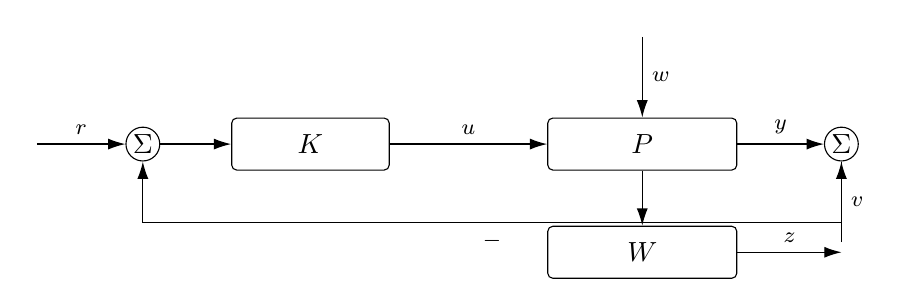
\begin{tikzpicture}[node distance=9mm]
      \node[smallbox, minimum width=20mm] (K) {$K$};
      \node[smallbox, right=20mm of K, minimum width=24mm] (P) {$P$};
      \node[sum, left=9mm of K] (sumin) {$\Sigma$};
      \node[sum, right=11mm of P] (sumy) {$\Sigma$};
      \draw[line] (sumin) -- (K);
      \draw[line] (K) -- node[above, font=\footnotesize] {$u$} (P);
      \draw[line] (P) -- node[above, font=\footnotesize] {$y$} (sumy);
      \draw[line] (sumy) |- ++(0,-10mm) -| node[pos=0.25, below, font=\footnotesize] {$-$} (sumin);
      \node[left=10mm of sumin] (r) {};
      \draw[line] (r.center) -- node[above, font=\footnotesize] {$r$} (sumin);
      \node[above=9mm of P] (w) {};
      \draw[line] (w.center) -- node[right, font=\footnotesize] {$w$} (P.north);
      \node[below=9mm of sumy] (v) {};
      \draw[line] (v.center) -- node[right, font=\footnotesize] {$v$} (sumy.south);
      \node[smallbox, below=7mm of P] (W) {$W$};
      \draw[line] (P.south) -- (W.north);
      \node[right=12mm of W] (z) {};
      \draw[line] (W) -- node[above, font=\footnotesize] {$z$} (z.center);
    \end{tikzpicture}}
    \caption{Closed-loop structure for $H_\infty$ design.}
    \label{fig:closed}
  \end{minipage}
\end{figure*}

\end{document}
